\documentclass{article}


\usepackage{arxiv}

\usepackage[utf8]{inputenc} % allow utf-8 input
\usepackage[T1]{fontenc}    % use 8-bit T1 fonts
\usepackage{hyperref}       % hyperlinks
\usepackage{url}            % simple URL typesetting
\usepackage{booktabs}       % professional-quality tables
\usepackage{amsfonts}       % blackboard math symbols
\usepackage{nicefrac}       % compact symbols for 1/2, etc.
\usepackage{microtype}      % microtypography
\usepackage{lipsum}
\usepackage{graphicx}
\usepackage{csquotes}

\graphicspath{ {./images/} }

\usepackage{fontsize}
\changefontsize{11}

\setlength{\parindent}{0pt} % Paragraph indentation
\setlength{\parskip}{0.8em} % Vertical space between paragraphs


\title{Analyse Détaillée de Mixture-of-Recursions (MoE)}


\author{
 Mokira \\
  % School of Coumputing and Information\\
  % University of Pittsburgh\\
  % Pittsburgh, PA 15213 \\
  % \texttt{dr.mokira@gmail.com} \\
  Ingénieur Machine Learning \\
  (+229) 019 798 5109 \\
  \texttt{dr.mokira@gmail.com} \\
  %% \AND
  %% Coauthor \\
  %% Affiliation \\
  %% Address \\
  %% \texttt{email} \\
  %% \And
  %% Coauthor \\
  %% Affiliation \\
  %% Address \\
  %% \texttt{email} \\
  %% \And
  %% Coauthor \\
  %% Affiliation \\
  %% Address \\
  %% \texttt{email} \\
}

\begin{document}
\maketitle
\begin{abstract}
Pourquoi MoR est une petite révolution ?
Imaginez un modèle de langage qui combine l’efficacité mémoire
des architectures à partage de paramètres (comme ALBERT) avec l’intelligence
computationnelle du calcul adaptatif (comme Mixture-of-Depths) :
c’est exactement ce que propose Mixture-of-Recursions (MoR).
Au lieu d’utiliser des couches distinctes, MoR réutilise un même bloc
de calcul de manière récursive, tandis qu’un routeur léger décide
dynamiquement pour chaque mot s’il doit « sortir » rapidement ou "réfléchir"
plus longtemps en passant par des recursions supplémentaires. Résultat ?
Une réduction simultanée de la taille du modèle (-50\% de paramètres),
du temps de calcul (meilleur débit d’inférence) et de la mémoire cache,
sans sacrifier la performance --- ouvrant la voie à des LLMs à la fois agiles,
économiques et puissants. Une avancée architecturale majeure qui mérite
d’être explorée dans les moindres détails !
\end{abstract}


% keywords can be removed
%\keywords{First keyword \and Second keyword \and More}


\section{Introduction}
Aujourd'hui, les intelligences artificielles qui comprennent et génèrent
du langage, comme celles qui animent les assistants virtuels, reposent
sur des architectures dites « Transformers ». Si elles sont impressionnantes,
leur formidable puissance a un coût : une gourmandise excessive en calcul
et en mémoire. Pour fonctionner, ces modèles doivent en effet traiter
chaque mot d'un texte avec la même intensité. Par exemple, pour comprendre
un mot complexe comme « philosophique », un modèle de langue doit lui accorder
autant de temps et de ressources qu’à un mot simple comme « le » ou « et ».
Cette approche uniforme est coûteuse et inefficace.

Les LLMs sont puissants, mais gourmands en mémoire et en calcul.
Et si on pouvait créer un modèle à la fois compact et intelligent,
capable de concentrer ses efforts sur les mots qui en valent vraiment
la peine ?

C'est la réponse à cette question qui a donné naissance
à la \textbf{Mixture-of-Recursions (MoR)}. une nouvelle architecture
qui permet à un modèle de langage d'allouer intelligemment son « effort
de calcul » de manière adaptive, token par token. Imaginez une usine
de traitement où les produits simples sont expédiés rapidement
après une étape, tandis que les produits complexes passent
par plusieurs stations de contrôle pour un travail approfondi.
MoR opère de la même façon : en réutilisant un même groupe de couches
de neurones de manière recursive, et en utilisant un mécanisme de décision
légère pour déterminer quels mots méritent plus de « réflexion ».
Cette méthode unifie pour la première fois les gains en efficacité
mémoire (moins de paramètres) et en efficacité computationnelle
(moins de calculs superflus), sans compromettre les performances.

Dans ce didacticiel, nous commencerons par un rappel des concepts
fondamentaux nécessaires à la compréhension. Ensuite, nous définirons
précisément le problème qui se pose. Puis, nous détaillerons
le fonctionnement de la solution proposée par MoR pour résoudre le problème,
Nous illustrerons cette solution par des exemples concrets
et une implémentation simplifiée en Python.
Nous discuterons ensuite des apports majeurs et des limites de cette solution,
et proposerons des pistes d'amélioration futures,
et enfin conclure sur la portée de ce travail.

\section{Connaissances de Base Nécessaires}
\label{sec:base}
Pour comprendre ce papier, il faut se familiariser avec quelques concepts
clés des modèles de type Transformers.

\subsection{Architecture Transformer de base (Vaswani et al., 2017)}
Un transformer est un modèle de réseau de neurones qui utilise
des \textbf{mécanismes d'attention} pour traiter des séquences de données
(comme du texte). Il est composé de couches (layers)
empilées les unes sur les autres. Chaque couche a une \textbf{auto-attention}
et un réseau \textbf{feed-forward}.

Imaginez un Transformer comme une usine avec plusieurs étages (couches/layers).
Chaque étage traite l'information et la passe à l'étage suivant.
Dans un modèle traditionnel comme GPT :

Entrée : "Le chat mange" $\rightarrow$ Couche $1$ $\rightarrow$ Couche $2$
$\rightarrow \ldots \rightarrow $  Couche $N$ → Sortie : "le poisson"

À chaque étage, chaque mot (token) regarde tous les autres mots pour mieux
se comprendre soi-même (c'est l'auto-attention), puis une petite usine interne
(le feed-forward) pour calculer sa représentation.

\subsection{Cache KV (Key-Value Cache)}
Pour générer du texte de manière autoregressive (un mot à la fois),
on doit éviter de recalculer les représentations des mots passés
à chaque nouvelle étape. Le cache KV stocke les "clés" et "valeurs" de tous
les mots déjà générés, ce qui rend le processus beaucoup plus rapide.

De façon analogique, lorsque vous lisez un livre, vous n'oubliez
pas les chapitres précédents. Votre cerveau garde en cache les informations
importantes. Le cache KV fait la même chose pour le modèle.

\subsection{Partage de Paramètres (Parameter Sharing)}
Au lieu d'avoir des poids uniques pour chaque couche, on utilise le même jeu
de poids pour plusieurs couches. Cela réduit énormément la taille du modèle.

Exemple : Au lieu d'avoir 24 stations de travail différentes dans notre usine,
on n'en a que 8, mais on fait passer la phrase 3 fois par les mêmes 8 stations.
L'usine est plus petite (moins de paramètres) mais le travail est tout aussi
profond (3 passages = 24 traitements effectifs).

\subsection{Calcul Adaptatif (Adaptive Computation)}
L'idée que tous les mots ne méritent pas le même effort de calcul.
Les mots de structure ("le", "la", "et") sont simples, tandis que les mots
de fond ("quantique", "philosophie") sont complexes. Le calcul adaptatif
permet au modèle de "réfléchir" plus longtemps aux mots difficiles.

\section{Le Problème posé}
Les modèles de langage (LLMs) comme GPT-4 sont très puissants
mais ont deux énormes défauts :

\begin{itemize}
  \item  Ils ont des milliards de paramètres, ce qui les rend très coûteux
  à entraîner et à stocker.
  \item Le mécanisme d'attention standard a une complexité quadratique $O(n^2)$.
  Pour générer de longues séquences, le calcul devient extrêmement lent
  et gourmand en énergie.
\end{itemize}

Les solutions existantes s'attaquent souvent à un seul de ces problèmes
à la fois.

\begin{itemize}
  \item \textit{ALBERT} réduit la taille du modèle mais applique
  le même nombre de calculs à tous les tokens (inefficient).
  \item \textit{Mixture-of-Depths} réduit le calcul pour les tokens
  "faciles" mais n'utilise pas de partage de paramètres, donc la taille
  du modèle reste grande.
\end{itemize}

Le problème fondamental est donc : Comment créer un modèle qui est à la fois
petit (grâce au partage de paramètres) et rapide à l'inférence
(grâce au calcul adaptatif) sans sacrifier la performance ?
C'est ce problème que MoR résout.


\section{La Solution : Mixture-of-Recursions (MoR)}
MoR est une architecture unifiée qui combine intelligemment le partage
de paramètres et le calcul adaptatif.

\subsection{Concept de Base}
 Au lieu d'empiler $24$ couches différentes, MoR a un petit bloc de $N$
 couches partagées (par exemple, $8$ couches). Ce bloc va être appliqué
 de manière répétée (récursive), jusqu'à $N_r$ fois (par exemple, $3$ fois).
 Le traitement effectif total est de $8 \times 3 = 24$ couches,
 mais on stocke que $8$ couches de paramètres. Ce qui nous permet d'économiser
 de la mémoire stockage.

 À la fin de chaque application du bloc récursif, un routeur léger décide
 pour chaque token s'il doit "sortir" (il a fini de réfléchir)
 ou s'il doit passer une nouvelle fois dans le bloc récursif (il a besoin
 de plus de réflexion). C'est le \textit{Routage Adaptatif par Token}
 (voir figure 1). Cela permet d'économiser en calcul sur des mots simples
 à comprendre.

\subsection{Expert choice routing}
Imaginez qu'on place un filtre à chaque sortie d'une couche.

\begin{enumerate}
  \item À la fin de la première étape de calcul, un "manager" (le routeur)
  évalue tous les coureurs et dit : "Seuls les $70\%$ qui ont le plus d'énergie
  continuent !". Les autres (les mots simples comme \texttt{"le"},
  \texttt{"la"}) quittent la piste.
  
  \item Les tokens restants font une deuxième tour. À la fin, le manager
  regarde à nouveau et dit : "Maintenant, seuls les $40\%$ meilleurs
  continuent !".

  \item Le processus se répète, en gardant de moins en moins de tokens
  à chaque fois.
\end{enumerate}

\begin{figure}[h]
  \centering
  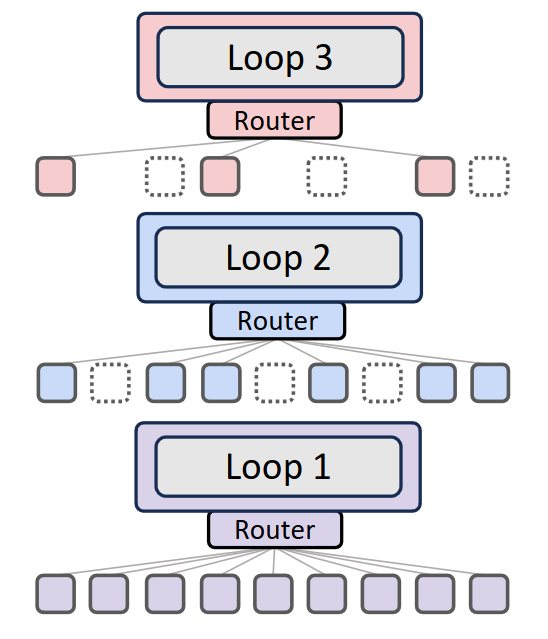
\includegraphics[scale=0.4]{images/expert_choice_routing.png}
  \caption{Routage par choix d'expert \cite{bae2025mixtureofrecursionslearningdynamicrecursive}}
  \label{fig:expert-choice-routing}
\end{figure}

Chaque "étape de récursion" agit comme un expert qui choisit les tokens
qu'il veut traiter. Ce qui permet un contrôle très précis du budget calcul
à chaque étape. On sait exactement combien de tokens sont actifs.

\subsection{Token choice routing}
Le token lui-même, via sa représentation initiale, "choisit" en quelque sorte
combien de calcul il va recevoir. Dès le début, un routeur regarde
la représentation de chaque token et en fonction de cela il assigne
une "profondeur de récursion" (nombre de tour).
 
 \begin{figure}[h]
  \centering
  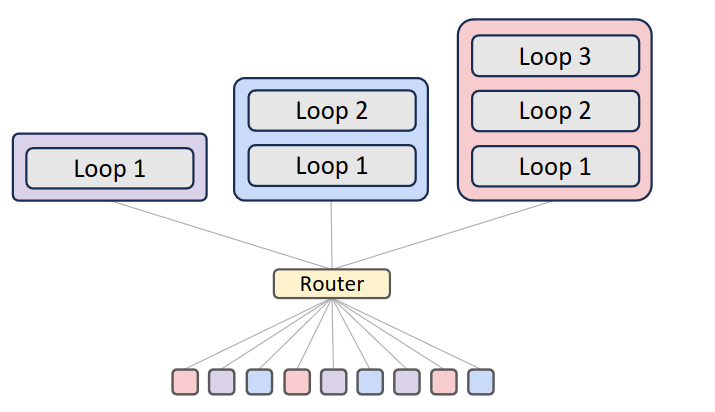
\includegraphics[scale=0.5]{images/token_choice_routing.png}
  \caption{Routage par choix du token \cite{bae2025mixtureofrecursionslearningdynamicrecursive}}
  \label{fig:token-choice-routing}
\end{figure}
 
 Prenons par exemple la phrase suivante :
 \texttt{"Le chat philosophique mange la nourriture délicate."}, pour chaque
 mot, en fonction de leur représentation, le routeur va décider immédiatement
 du nombre de tours qu'il fera.
 
 \begin{itemize}
  \item \texttt{"Le"}, \texttt{"la"} ---> $1$ recursion
  (sort immédiatement après le premier passage, c'est un mot de structure);
  \item \texttt{"chat"}, \texttt{"mange"}, \texttt{"nourriture}" ---> $2$ tours
  (mots normaux);
  \item \texttt{"philosophique"}, \texttt{"délicate"} ---> $3$ tours
  (mots complexes qui nécessitent une "réflexion" profonde).
 \end{itemize}

 À la fin du permier passage, le routeur sélectionne \texttt{"philosophique"},
 \texttt{"délicate"}, \texttt{"chat"}, \texttt{"mange"}. \texttt{"Le"}
 et \texttt{"la"} sortent. Ensuite, à la fin du 2ème passage, le routeur
 sélectionne \texttt{"philosophique"} et \texttt{"délicate"}.
 Les autres sortent. Au 3ème passage, seuls les deux mots complexes restants
 terminent leur traitement.

 Chaque token parcourt le nombre de boucles qui lui a été assigné,
 puis s'arrête. Il n'y a pas de décision à prendre après le départ.
 En effet, c'est le token lui-même, via sa représentation initiale,
 qui "choisit" en quelque sorte combien de calcul il va recevoir.

Les mots simples ont été calculés rapidement, libérant les ressources
pour que le modèle réfléchisse longuement aux mots complexes.
Tout cela en réutilisant le même petit bloc de couches.


%  \cite{bae2025mixtureofrecursionslearningdynamicrecursive}




\subsection{Headings: second level}
\lipsum[5]
\begin{equation}
\xi _{ij}(t)=P(x_{t}=i,x_{t+1}=j|y,v,w;\theta)= {\frac {\alpha _{i}(t)a^{w_t}_{ij}\beta _{j}(t+1)b^{v_{t+1}}_{j}(y_{t+1})}{\sum _{i=1}^{N} \sum _{j=1}^{N} \alpha _{i}(t)a^{w_t}_{ij}\beta _{j}(t+1)b^{v_{t+1}}_{j}(y_{t+1})}}
\end{equation}

\subsubsection{Headings: third level}
\lipsum[6]

\paragraph{Paragraph}
\lipsum[7]

\section{Examples of citations, figures, tables, references}
\label{sec:others}
\lipsum[8] \cite{kour2014real,kour2014fast} and see \cite{hadash2018estimate}.

The documentation for \verb+natbib+ may be found at
\begin{center}
  \url{http://mirrors.ctan.org/macros/latex/contrib/natbib/natnotes.pdf}
\end{center}
Of note is the command \verb+\citet+, which produces citations
appropriate for use in inline text.  For example,
\begin{verbatim}
   \citet{hasselmo} investigated\dots
\end{verbatim}
produces
\begin{quote}
  Hasselmo, et al.\ (1995) investigated\dots
\end{quote}

\begin{center}
  \url{https://www.ctan.org/pkg/booktabs}
\end{center}


\subsection{Figures}
\lipsum[10]
See Figure \ref{fig:fig1}. Here is how you add footnotes. \footnote{Sample of the first footnote.}
\lipsum[11]

\begin{figure}
  \centering
  \fbox{\rule[-.5cm]{4cm}{4cm} \rule[-.5cm]{4cm}{0cm}}
  \caption{Sample figure caption.}
  \label{fig:fig1}
\end{figure}

\begin{figure} % picture
    \centering
    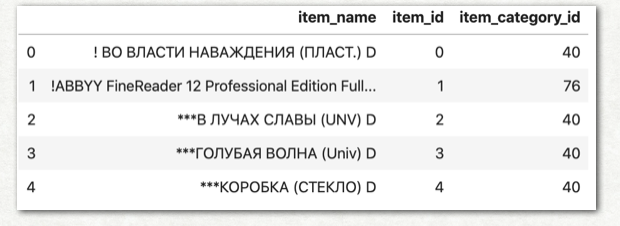
\includegraphics{test.png}
\end{figure}

\subsection{Tables}
\lipsum[12]
See awesome Table~\ref{tab:table}.

\begin{table}
 \caption{Sample table title}
  \centering
  \begin{tabular}{lll}
    \toprule
    \multicolumn{2}{c}{Part}                   \\
    \cmidrule(r){1-2}
    Name     & Description     & Size ($\mu$m) \\
    \midrule
    Dendrite & Input terminal  & $\sim$100     \\
    Axon     & Output terminal & $\sim$10      \\
    Soma     & Cell body       & up to $10^6$  \\
    \bottomrule
  \end{tabular}
  \label{tab:table}
\end{table}

\subsection{Lists}
\begin{itemize}
\item Lorem ipsum dolor sit amet
\item consectetur adipiscing elit.
\item Aliquam dignissim blandit est, in dictum tortor gravida eget. In ac rutrum magna.
\end{itemize}


\bibliographystyle{unsrt}
\bibliography{references}  %%% Remove comment to use the external .bib file (using bibtex).
%%% and comment out the ``thebibliography'' section.


%%% Comment out this section when you \bibliography{references} is enabled.
% \begin{thebibliography}{1}

% \bibitem{kour2014real}
% George Kour and Raid Saabne.
% \newblock Real-time segmentation of on-line handwritten arabic script.
% \newblock In {\em Frontiers in Handwriting Recognition (ICFHR), 2014 14th
%   International Conference on}, pages 417--422. IEEE, 2014.

% \bibitem{kour2014fast}
% George Kour and Raid Saabne.
% \newblock Fast classification of handwritten on-line arabic characters.
% \newblock In {\em Soft Computing and Pattern Recognition (SoCPaR), 2014 6th
%   International Conference of}, pages 312--318. IEEE, 2014.

% \bibitem{hadash2018estimate}
% Guy Hadash, Einat Kermany, Boaz Carmeli, Ofer Lavi, George Kour, and Alon
%   Jacovi.
% \newblock Estimate and replace: A novel approach to integrating deep neural
%   networks with existing applications.
% \newblock {\em arXiv preprint arXiv:1804.09028}, 2018.

% \end{thebibliography}


\end{document}
